%
% versuch.tex -- Paper zum Thema Optische Fourier-Transformation <opt>
%
% (c) 2023 Marco Niederberger, Yanick Schoch; OST Ostschweizer Fachhochschule
%
% !TEX root = ../../buch.tex
% !TEX encoding = UTF-8
%
\section{Versuch
  \label{opt:section:versuch}}
\rhead{Praktische Erprobung}

Der durchgeführte Versuch entspricht im Aufbau demjenigen aus Abbildung \ref{opt:fig:4fAufbau}.
Für die Fourier-Transformation wurden eine Linse mit 300 mm Brennweite genutzt, damit war der Effekt am besten sichtbar.
Der vorhandene Helium-Neon-Laser erzeugt einen Laserstrahl mit einem Durchmesser von $0.8$ mm.
\index{Helium-Neon-Laser}%
\index{Laser}%
Um die gerade Wellenfront in ausreichendem Durchmesser zu erhalten, wurde der Strahl mittels eines umgekehrten keplerschen Teleskops aufgeweitet.
\index{keplersches Teleskop}%
\index{Teleskop, keplersch}%
Der schematische Aufbau ist in Abbildung \ref{opt:fig:laserAufweiten} ersichtlich.
Dafür wird direkt hinter der Laserblende eine konkave Linse mit einer Brennweite $f_b = 50\,\text{mm}$ montiert 
und in einem Abstand von $f_b + f_o = 200\,\text{mm}$ eine weitere mit einer Brennweite von $f_o = 150\,\text{mm}$.
Somit wird der Laserstrahl um ein Faktor $\frac{f_o}{f_b} = 3$ vergrössert.
Dies war ausreichend, um die vorhandenen Blenden vollständig auszuleuchten.

Anschliessend konnte eine erste Blende montiert werden.
In Abbildung \ref{opt:fig:4fAufbau} ist dies als Originalbild beschrieben.
Im Abstand $f=300\,\text{mm}$ wird jetzt die erste Linse montiert und nach weiteren zwei Brennweiten die zweite Linse.
Genau in der Mitte der beiden Linsen ergibt sich die Fourier-Ebene.
Ganz am Ende des Aufbaus, eine weitere Brennweite hinter der zweiten Linse, ist das rücktransformierte Bild ersichtlich.

Im weiteren Verlauf dieses Abschnittes werden die erwarteten Ergebnisse simuliert und anschliessend mit den Beobachtungen verglichen.

\subsection{Simulation der erwarteten Ergebnissen}
Der $4f$ Versuch kann auch simuliert werden.
\index{4f Versuch@$4f$ Versuch}%
In unserem Fall geschah dies mit \emph{Python} und der \emph{numpy} Bibliothek.
\index{numpy}%
\index{Python}%
Zuerst wird ein Input-Bild erstellt, welches anschliessend bearbeitet wird.
Als Input wurden ein Dreifachspalt sowie ein Gitter verwendet.
Mittels zweidimensionaler diskreter Fast-Fourier-Transformation (FFT) wird das Originalbild in den Frequenzbereich transformiert.
Anschliessend kann dies mit einem digitalen Filter gefiltert werden.
Die Filter werden so ausgeführt, wie sie in Abbildung \ref{opt:fig:filterarten} aufgeführt sind.
Das bedeutet, dass zum Beispiel ein Tiefpass einen runden Durchlassbereich um den Nullpunkt hat.
Schlussendlich wird das gefilterte Frequenzspektrum mittels zweidimensionaler FFT wieder rücktransformiert.
Abbildung \ref{opt:fig:three_slit_simulation} zeigt diesen Vorgang am Beispiel eines Dreifachspalts und 
in Abbildung \ref{opt:fig:grid_simulation} wird dasselbe mit einem Gitter simuliert.

Die verwendeten Python-Skripte der Simulation sind im Repository des Buches\footnote{\url{https://github.com/AndreasFMueller/SeminarHarmonischeAnalysis/tree/master/buch/papers/opt/code}}
abgelegt.

\subsection{Versuchsdurchführung}
Zuerst wurde die Funktion des Aufbaus mit einem $2f$ Versuch verifiziert.
Dabei wird nur eine Linse aus dem $4f$ Aufbau verwendet und das entstandene Spektrum wird im Abstand der Brennweite betrachtet.
Die dabei entstandenen Bilder entsprachen den Erwartungen.
Für den Einzelspalt war, wie in Abschnitt \ref{opt:sec:exampleSingleSlit} berechnet, eine sinc-förmige Verteilung der Intensität zu betrachten.

Nach dieser Verifizierung wurde die zweite Linse ebenfalls montiert und die Abbildungsebene hinter die zweite Linse gelegt.
Beim Dreifachspalt konnte die Fourier-Transformation und Rücktransformation erfolgreich ausgeführt werden.
Die Filterung mittels eines optischen Tiefpasses konnte jedoch nicht nachgebildet werden.
Der genaue Grund dafür konnte nicht eruiert werden.
Mögliche Ursachen sind eine zu grosse Blende, eine nicht optimale Ausrichtung der optischen Achse oder eine zu geringe Auflösung der Auswerteeinheit.

\subsection{Vergleich der Simulation}
In der Abbildung \ref{opt:fig:experiment} sind die Resultate aus dem Versuch mit dem Dreifachspalt ersichtlich.
Wenn das erhaltene Spektrum mit demjenigen aus der Simulation in Abbildung \ref{opt:fig:three_slit_simulation} verglichen wird, ist eine Übereinstimmung ersichtlich.
In beiden Fällen ist auf der $x$-Achse eine erhöhte Intensität zu beobachten mit einem grossen Anteil im Ursprung.
Ebenfalls in beiden Fällen kann auch auf der $y$-Achse eine kleine Intensität beobachtet werden.
Diese folgt davon, dass der Spalt eine beschränkte Dimension in der $y$-Richtung hat und somit auch dort die Welle gebeugt wird.
Beim reellen Versuch können noch weitere Bereiche mit einer sichtbaren Intensität ausgemacht werden, welche in der Simulation nicht ersichtlich sind.
Dies war jedoch zu erwarten, da die Simulation im Gegensatz zum realen Versuchsaufbau viel genauer ist und sich nicht durch Störungen im Aufbau beeinflussen lässt.


\begin{figure}
    \centering
    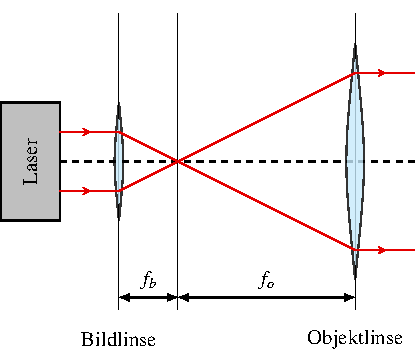
\includegraphics[width=60mm]{papers/opt/images/laserAufweiten.pdf}
    \caption{Die Vergrösserung des Laserlichts erfolgt mit einem Kepler-Teleskop.
        Dazu werden zwei Linsen mit unterschiedlichen Brennweiten verwendet.
\index{keplersches Teleskop}%
        Der Abstand dazwischen ist die Summe der beiden Brennweiten.}
    \label{opt:fig:laserAufweiten}
\end{figure}

\begin{figure}
    \centering
    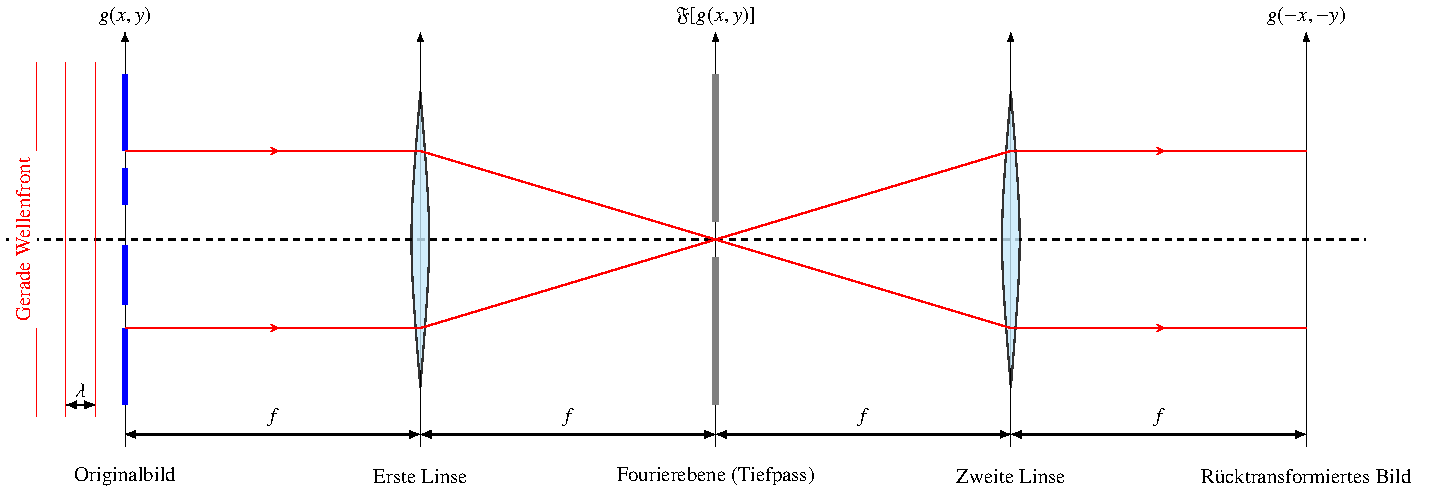
\includegraphics[width=\textwidth]{papers/opt/images/4fAufbau.pdf}
    \caption{Der $4f$ Aufbau ermöglicht eine Fourier-Transformation des Originalbildes sowie eine Rücktransformation aus der Fourier-Ebene.
\index{Fourier-Ebene}%
    In dieser Abbildung wird die transformierte Funktion mit einem Tiefpass gefiltert.
\index{Tiefpass}%
    Weitere Details zu den Filtern folgen im Abschnitt \ref{opt:section:filter}.}
    \label{opt:fig:4fAufbau}
\end{figure}

\begin{figure}
    \centering
    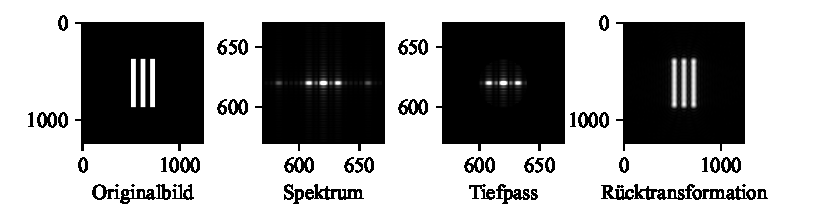
\includegraphics[width=\textwidth]{papers/opt/images/dreifachspalt_tiefpass.pdf}
    \caption{Der Dreifachspalt wird zunächst fouriertransformiert, dann mit einem Tiefpass gefiltert und wieder rücktransformiert.
    Die ursprünglich scharfen Kanten des Spalts werden dadurch unscharf wiedergegeben.}
    \label{opt:fig:three_slit_simulation}
\end{figure}

\begin{figure}
    \centering
    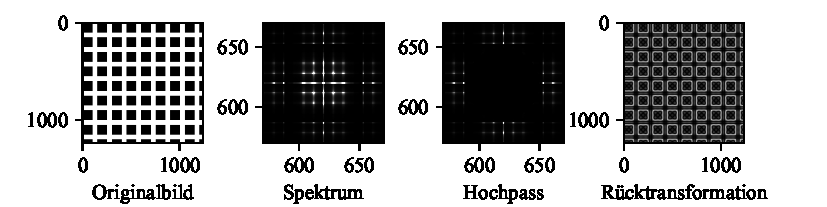
\includegraphics[width=\textwidth]{papers/opt/images/gitter_hochpass.pdf}
    \caption{Das Gitter wird zunächst fouriertransformiert, dann mit einem Hochpass gefiltert und wieder rücktransformiert.
    In der Rücktransformation sind insbesondere die harten Kanten des Gitters erkennbar.}
    \label{opt:fig:grid_simulation}
\end{figure}

\begin{figure}
    \centering
    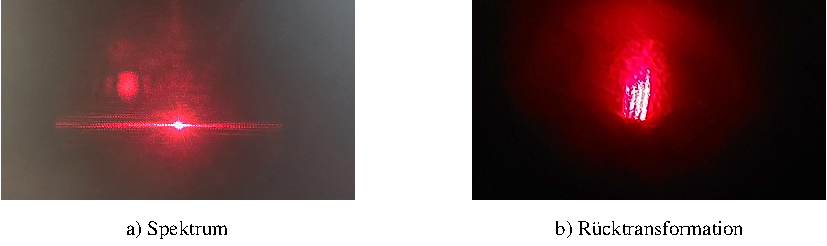
\includegraphics[width=\textwidth]{papers/opt/images/experiment.pdf}
    \caption{Der $4f$ Versuch aus dem Abschnitt \ref{opt:section:versuch} wurde hier mit einem Dreifachspalt durchgeführt.
    Abbildung a) zeigt das daraus entstandene Spektrum und in der Abbildung b) ist die Rücktransformation davon zu sehen.}
    \label{opt:fig:experiment}
\end{figure}
